%% Direttive TeXworks:
% !TeX root = ../maltoni_niccolo_tesi.tex
% !TEX encoding = UTF-8 Unicode
% !TEX program = arara
% !TEX TS-program = arara
% !TeX spellcheck = it-IT

%% Direttive Arara:
% arara: pdflatex: { shell: yes, synctex: yes, action: batchmode, options: "-halt-on-error -file-line-error-style" }
% arara: frontespizio
% arara: biber
% arara: pdflatex: { shell: yes, synctex: yes, action: batchmode, options: "-halt-on-error -file-line-error-style" }
% arara: pdflatex: { shell: yes, synctex: yes, action: nonstopmode, options: "-halt-on-error -file-line-error-style" }

\chapter{Introduzione}\label{ch:intro}

    \section{Alchemist}\label{sec:alchemist}
        Alchemist~\cite{alchemistWeb, alchemist2013} è un meta-simulatore estendibile completamente \engEmph{open-source} che esegue su Java Virtual Machine (JVM), nato all'interno del'Università di Bologna e distribuito su licenza GNU GPLv3+ con \engEmph{linking exception}; il codice è reperibile su GitHub\footnote{\url{https://github.com/AlchemistSimulator/Alchemist}}\label{fn:gh}, dove chiunque fosse interessato può collaborare sviluppando nuove estensioni, migliorando funzionalità esistenti e risolvendo possibili bug.

        \subsection{Introduzione ad Alchemist}\label{sub:introAlchemist}
            In generale, una \emph{simulazione}~\cite{des3} è una riproduzione del modo di operare di un sistema o un processo del mondo reale nel tempo.
            L'imitazione del processo del mondo reale è detta \emph{modello}; esso risulta essere una riproduzione più o meno semplificata del mondo reale, che viene aggiornata ad ogni passo di esecuzione della simulazione.

            Alchemist rientra nell'archetipo dei simulatori ad eventi discreti (DES)~\cite{des, des2}: gli eventi sono strettamente ordinati e vengono eseguiti uno alla volta, mentre il tempo viene fatto avanzare parallelamente ad ogni passo (detto \engEmph{tick}).
            L'idea dietro al progetto è quello di riuscire ad avere un framework di simulazione il più possibile generico, in grado di simulare sistemi di tipologia e complessità diverse, mantenendo le prestazioni dei simulatori non generici (come ad esempio quelli impiegati in ambito chimico~\cite{gillespie1976}).

            Per perseguire questo obiettivo, la progettazione dell'algoritmo è partita dal lavoro di Gillespie del 1977~\cite{gillespie1977}, al quale sono state aggiunte diverse modifiche per adattarlo al rinnovato metamodello.

            % TODO aggiungi qualche riferimento al Next Reaction Method (Gibson and Bruck, 2000).

        \subsection{Modello computazionale di Alchemist}\label{sub:modelloComputazionale}
            Il modello (visibile in \figurename~\vref{fig:model}) che costituisce l'architettura base di Alchemist è, come detto, ispirato ad algoritmi tipici della simulazione a scopo di ricerca chimica e, dunque, ne riprende la nomenclatura, seppur con alcune libertà atte ad ottenere una maggiore flessibilità.
            Le entità su cui lavora sono le seguenti:
            \begin{description}

                \item[\engEmph{Molecule}\label{itm:mol}]
                    Una \emph{Molecola} rappresenta il nome dato ad un particolare dato all'interno di un \emph{Nodo}, del quale ne astrae parte dello stato.

                    Un parallelismo con la programmazione imperativa vedrebbe la \emph{Molecola} come un'astrazione del nome di una variabile.

                \item[\engEmph{Concentration}\label{itm:conc}]
                    La \emph{Concentrazione} di una \emph{Molecola} è il valore associato alla proprietà rappresentata dalla \emph{Molecola}.

                    Mantenendo il parallelismo con la programmazione imperativa, la \emph{Concentrazione} rappresenterebbe il valore della variabile.

                \item[\engEmph{Node}\label{itm:node}]
                    Il \emph{Nodo} è un contenitore di \emph{Molecole} e \emph{Reazioni} che risiede all'interno di un \emph{Ambiente} e che astrae una singola entità.

                \item[\engEmph{Environment}\label{itm:env}]
                    L'\emph{Ambiente} è l'astrazione che rappresenta lo spazio nella simulazione ed è l'entità che contiene i nodi.

                    Esso è in grado di fonrire informazioni in merito alla posizione dei \emph{Nodi} nello spazio, alla distanza tra loro e al loro vicinato; opzionalmente, l'\emph{Ambiente} può offrire il supporto allo spostamento dei \emph{Nodi}.

                \item[\engEmph{Linking rule}\label{itm:linkr}]
                    La \emph{Regola di collegamento} è la funzione dello stato corrente dell'\emph{Ambiente} che associa ad ogni \emph{Nodo} un \emph{Vicinato}.

                \item[\engEmph{Vicinato}\label{itm:neigh}]
                    Un \emph{Vicinato} è un'entità costituita da un \emph{Nodo} detto ''centro'' e da un insieme di altri \emph{Nodi} (i ''vicini'').

                    L'astrazione dovrebbe avere un'accezione il più possibile generale e flessibile, in modo da poter modellare qualsiasi tipo di legame di vicinato, non solo spaziale.

                    \begin{figure}[htbp]\label{fig:model}
                        \centering
                        \includegraphics[scale=.4]{img/model}
                        \caption{%
                            La figura, presa dal sito ufficiale~\cite{alchemistWeb}, offre una rappresentazione grafica delle diverse entità. All’interno di un ambiente, che modella il sistema, si trovano i nodi connessi tra loro attraverso dei collegamenti; ogni nodo è composto da reazioni e molecole, ognuna delle quali ha associata una concentrazione.
                        }
                    \end{figure}

                \item[\engEmph{Reaction}\label{itm:react}]
                    Il concetto di \emph{Reazione} è da considerarsi molto più elaborato di quello utilizzato in chimica: in questo caso, si può considerare com un insieme di \emph{Condizioni} sullo stato del sistema, che qualora dovessero risultare vere innescherebbero l'esecuzione di un insieme di \emph{Azioni}.

                    Una \emph{Reazione} è dunque un qualsiasi evento che può cambiare lo stato dell’\emph{Ambiente} e si compone di un insieme di condizioni, una o più azioni e una distribuzione temporale.

                    La frequenza di accadimento può dipendere da:
                    \begin{itemize}
                        \item[--] Un tasso statico;
                        \item[--] Il valore di ciascuna \emph{Condizione};
                        \item[--] Una equazione che combina il tasso statico e il valore delle \emph{Condizioni}, restituendo un ''tasso istantaneo'';
                        \item[--] Una distribuzione temporale.
                    \end{itemize}

                    Ogni \emph{Nodo} è costituito da un insieme (anche vuoto) di \emph{Reazioni}.

                \item[\engEmph{Condition}\label{itm:cond}]
                    Una \emph{Condizione} è una funzione che associa un valore numerico e un valore booleano allo stato corrente di un \emph{Ambiente}.

                \item[\engEmph{Action}\label{itm:act}]
                        Un'\emph{Azione} è una procedura che provoca una modifica allo stato dell'\emph{Ambiente}.
            \end{description}

        \subsection{Interfaccia utente classica}\label{sub:prevGui}
            \subsubsection{Esperienza utente}\label{subsub:prevUx}
            \subsubsection{Swing}\label{subsub:swing}
            \subsubsection{Gli effetti e l'interfaccia \texttt{Effect}}\label{subsub:effect}
    \section{JavaFX}\label{sec:jfx}
        \subsection{Introduzione a JavaFX}\label{sub:jfxIntro}
        \subsection{Il framework JavaFX}\label{sub:jfxFramework}
        \subsection{Struttura di una Applicazione JavaFX}\label{sub:jfxStruttura}
        \subsection{Vantaggi di JavaFX su Swing}\label{sub:jfxVantaggi}
    \section{Interfaccia JavaFX per Alchemist: motivazioni}\label{sec:motivi}
